\chapter{Datový model}
	Tato kapitola se zabývá podrobnostmi o datovém modelu nástroje. Pojednává o volbě reprezentace kontraktů, které byly použity pro tento projekt a obecně o společných atributech kontraktů. Jsou zde uvedeny podrobnosti o datovém modelu určeném pro reprezentaci kontraktů, ale také pro výsledky jejich porovnání. Oba tyto modely jsou zde popsány slovně, ale i pomocí UML diagramu. Závěr tvoří informace o externí reprezentaci těchto dat.

	\section{Volba DbC konstrukcí}
		Po analýze dostupných materiálů jsem se rozhodl zvolit pro implementaci konstrukce Guava Preconditions a JSR305. Důvodem byla především jejich rozdílná reprezentace, kdy Guava Preconditions je realizováno pomocí volání metod uvnitř těl metod a umožňuje vytvářet vstupní podmínky. Na druhé straně JSR305 je tvořené anotacemi v záhlaví tříd, metod a také jako součást parametrů metod. Umožňuje tvoření všech tří typů kontraktů (vstupní, výstupní i neměnné podmínky). Kromě této diverzity se také jedná o jedny z častých konstrukcí používaných v projektech viz \cite{contractsInWild}. Principy obou těchto nástrojů byly již popsány výše (viz 3. kapitola Popis kontraktů softwarových rozhraní) z čehož se bude vycházet.
				
	\section{Společné znaky reprezentací kontraktů}		
		Při rozboru jednotlivých nástrojů pro reprezentaci design by contract zjistíme, že sdílejí mnoho podobných aspektů, které jsou klíčové pro vytvoření obecného modelu, který je schopen zachytit libovolnou konstrukci tohoto kontraktu. 
		
		TODO - doplnit společné znaky
	
	\section{Model pro extrakci kontraktů}
			TODO - úvod ... je potřeba data uložit atd.			
			
			Výsledný model jsem vytvořil na základě analýzy konstrukcí kontraktů s ohledem na následný export do dat, které bude možné dále zpracovávat. Aby byl zachován kontext kontraktů, usoudil jsem, že bude třeba zachovávat také informace o třídách a metodách v daném souboru. Rozhodl jsem se tedy vytvořit strukturu podobnou stromu, jejíž kořenem je samotný zdrojový soubor. Tento soubor obsahuje různé podrobnosti o tomto souboru jako je jeho jméno a cesta, typ a statistiky o jeho obsahu. Také obsahuje seznam všech tříd obsažených v tomto souboru.\\
			
			Každá jednotlivá třída pak obsahuje jméno, svou hlavičku, seznam metod a také seznam všech kontraktů týkajících se této třídy, tedy class invariants. Metoda pak nese informaci o své signatuře a také seznam všech kontraktů této metody. Samotný kontrakt pak obsahuje informaci o tom, o jaký typ kontraktu se jedná, o jakou podmínku se jedná, kompletní výraz a také jeho dílčí části.
			
			
			%%%%%%%%%%%%%%%%%%%%%%%%%%%%%%%%%%%%%%%%%%%%%%%%%%%%%%%%%%%%%%%%%%%%%%%%%%%%%%%%%%%%%%%%%%%%%%%%%%%%%%%%%%%%%%%%%%%%%%%%%%%%%%%%%%%%%%%%%%%%%%%%%%%%%%%%%%%%%%%%%%%%%%%%%%%%%%%%%%%%%%
			\subsection{Třída \texttt{JavaFile}}
				Instance této třídy představují samotné soubory. Zde je jeho kompletní struktura:
				
				\subsubsection{\texttt{String fileName}}	
					Jméno daného souboru bez cesty a bez koncovky.
					
				\subsubsection{\texttt{String fullPath}}
					Tento atribut obsahuje absolutní cestu k analyzovanému souboru.
					
				\subsubsection{\texttt{String shortPath}}
					Tato zkrácená cesta je použita při zpracování více souborů. Je pak uchována pouze rozdílná část těchto cest. To umožňuje přehlednější zobrazení v uživatelské aplikaci. Příkladem mohou být soubory, které mají tyto absolutní cesty: \texttt{C:/files/test/base/alpha.java} a \texttt{C:/files/test/common/beta.java}. Zkrácené cesty pak vypadají takto: \texttt{base/alpha.java} a \texttt{common/beta.java}.
					
				\subsubsection{\texttt{FileType fileType}}
					Atribut \texttt{fileType} je výčtový typ, který představuje typ daného souboru. Může se jednat o \texttt{JAVA} pro soubory \texttt{.java} a \texttt{CLASS} pro soubory \texttt{.class}.
					
				\subsubsection{\texttt{JavaFileStatistics javaFileStatistics}}
					Tento objekt obsahuje statistické údaje o daném souboru. je zde uložen počet tříd a metod. Také zde je počet metod s kontrakty a také celkový i dílčí počet všech kontraktů.
					
				\subsubsection{\texttt{List<JavaClass> javaClasses}}
					Zde, v seznamu objektů \texttt{JavaClass} (viz níže), jsou uloženy jednotlivé třídy, které jsou v daném souboru obsaženy.
			
			
			%%%%%%%%%%%%%%%%%%%%%%%%%%%%%%%%%%%%%%%%%%%%%%%%%%%%%%%%%%%%%%%%%%%%%%%%%%%%%%%%%%%%%%%%%%%%%%%%%%%%%%%%%%%%%%%%%%%%%%%%%%%%%%%%%%%%%%%%%%%%%%%%%%%%%%%%%%%%%%%%%%%%%%%%%%%%%%%%%%%%%%
			\subsection{Třída \texttt{JavaClass}}
				Instance \texttt{JavaClass} představují jednotlivé třídy v daném souboru.
				
				\subsubsection{\texttt{String name}}				
					Obsahuje jméno dané třídy.
			
				\subsubsection{\texttt{String signature}}				
					Představuje signaturu dané třídy a mimo názvu obsahuje také ostatní podrobnosti.
					
				\subsubsection{\texttt{List<JavaMethod> javaMethods}}
					Seznam objektů \texttt{JavaMethod} (viz níže), které reprezentují metody této třídy.
					
				\subsubsection{\texttt{List<Contract> invariants}}
					Seznam objektů typu \texttt{Contract} (viz níže), které představují neměnné proměnné této třídy.
			
			
			%%%%%%%%%%%%%%%%%%%%%%%%%%%%%%%%%%%%%%%%%%%%%%%%%%%%%%%%%%%%%%%%%%%%%%%%%%%%%%%%%%%%%%%%%%%%%%%%%%%%%%%%%%%%%%%%%%%%%%%%%%%%%%%%%%%%%%%%%%%%%%%%%%%%%%%%%%%%%%%%%%%%%%%%%%%%%%%%%%%%%%
			\subsection{Třída \texttt{JavaMethod}}
				Objekty typu \texttt{JavaMethod} reprezentují metody v nadřazené třídě.
				
				\subsubsection{\texttt{String signature}}
					Signatura této metody, která mimo jiné obsahuje návratový typ, název a vstupní parametry.
					
				\subsubsection{\texttt{boolean isConstructor}}
					Určuje, zda daná metoda je konstruktor, či se jedná o běžnou metodu.
					
				\subsubsection{\texttt{List<Contract> contracts}}
					Seznam objektů typu \texttt{Contract} (viz níže), které představují dílčí kontrakty dané metody. Jsou definovány vstupními i výstupními podmínkami.
						
			
			%%%%%%%%%%%%%%%%%%%%%%%%%%%%%%%%%%%%%%%%%%%%%%%%%%%%%%%%%%%%%%%%%%%%%%%%%%%%%%%%%%%%%%%%%%%%%%%%%%%%%%%%%%%%%%%%%%%%%%%%%%%%%%%%%%%%%%%%%%%%%%%%%%%%%%%%%%%%%%%%%%%%%%%%%%%%%%%%%%%%%%
			\subsection{Třída \texttt{Contract}}			
			
				\subsubsection{\texttt{ContractType contractType}} 
					Jedná se o výčtový typ, který určuje o jaký druh kontraktu se jedná. Při současném stavu knihovny to mohou být hodnoty Guava či JSR305.
			
				\subsubsection{\texttt{ConditionType conditionType}} 
					Opět výčtový typ který určuje typ kontraktu dle jeho podmínky. Rozlišují se tři druhy: \texttt{PRE} pro vstupní podmínku, \texttt{POST} pro výstupní podmínku a \texttt{INVARIANT} pro neměnnou podmínku.
			
				\subsubsection{\texttt{String completeExpression}} 
					Reprezentuje kompletní výraz celého kontraktu. I přesto, že celý výraz je možné vytvořit z jeho dílčích částí, je zde uveden pro rychlý přehled. Může také posloužit jako kontrola parsování či pro rychlé porovnání.
			
				\subsubsection{\texttt{String function}} 
					Tento řetězec určuje funkci o jakou se jedná v rámci daného kontratku. V případě Guava se jedná o název metody, v případě JSR305 o název anotace. Obecně se jedná o hlavní označení určující daný kontrakt.
			
				\subsubsection{\texttt{String expression}} 
					Obsahuje první parametr dané funkce. Důvodem, proč oddělit první parametr od ostatních, bylo, že kontrakty mají často pouze jeden parametr a pokud jich mají více, ostatní často nejsou tolik relevantní. Pro zvýšení přehlednosti byl tedy tento parametr uveden samostatně.
			
				\subsubsection{\texttt{List<String> arguments}} 
					Seznam ostatních argumentů daného kontraktu. Ostatní atributy až na výjimky slouží pouze k uvedení chybové zprávy, která se má zobrazit při porušení kontraktu. Mimo zprávy zde také bývají proměnné použité ve zprávě.\\					
	
		Během zpracování jsou používány následující třídy: \texttt{ExtendedJavaFile}, \texttt{ExtendedJavaClass} a \texttt{ExtendedJavaMethod}. Ty obsahují dodatečné informace vůči výše zmíněným objektům. Jedná se o anotace, vstupní parametry a jednotlivé části těl metod.	Po zpracování jsou pak tyto objekty redukovány na ty výše zmíněné, které jsou připraveny pro externí reprezentaci.
		
		
		\section{Diagram modelu pro extrakci kontraktů}
			Na obrázku \ref{modelExtractorDiagram} je vidět grafické znázornění datového modelu formou UML diagramu. Nejsou zde záměrně zobrazeny objekty \texttt{ContractComparison} a \texttt{JavaFileCompareReport}. Těm je věnován prostor v diagramu pro porovnávání kontraktů, který je na obrázku \ref{modelComparatorDiagram}.		
		
				\begin{figure}[!htb]
					\minipage{1\textwidth}	
						\centering
						%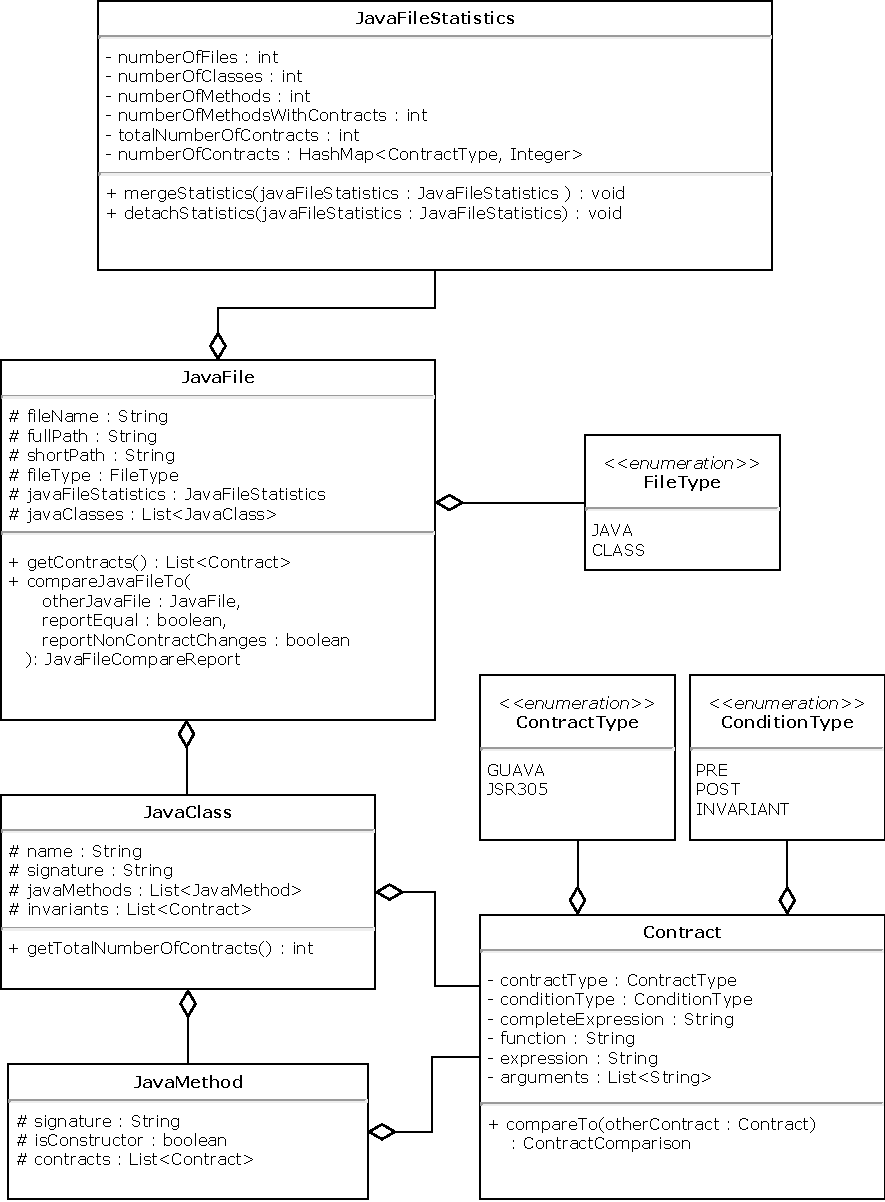
\includegraphics[width=1\textwidth]{img/modelExtractorDiagram.png}
						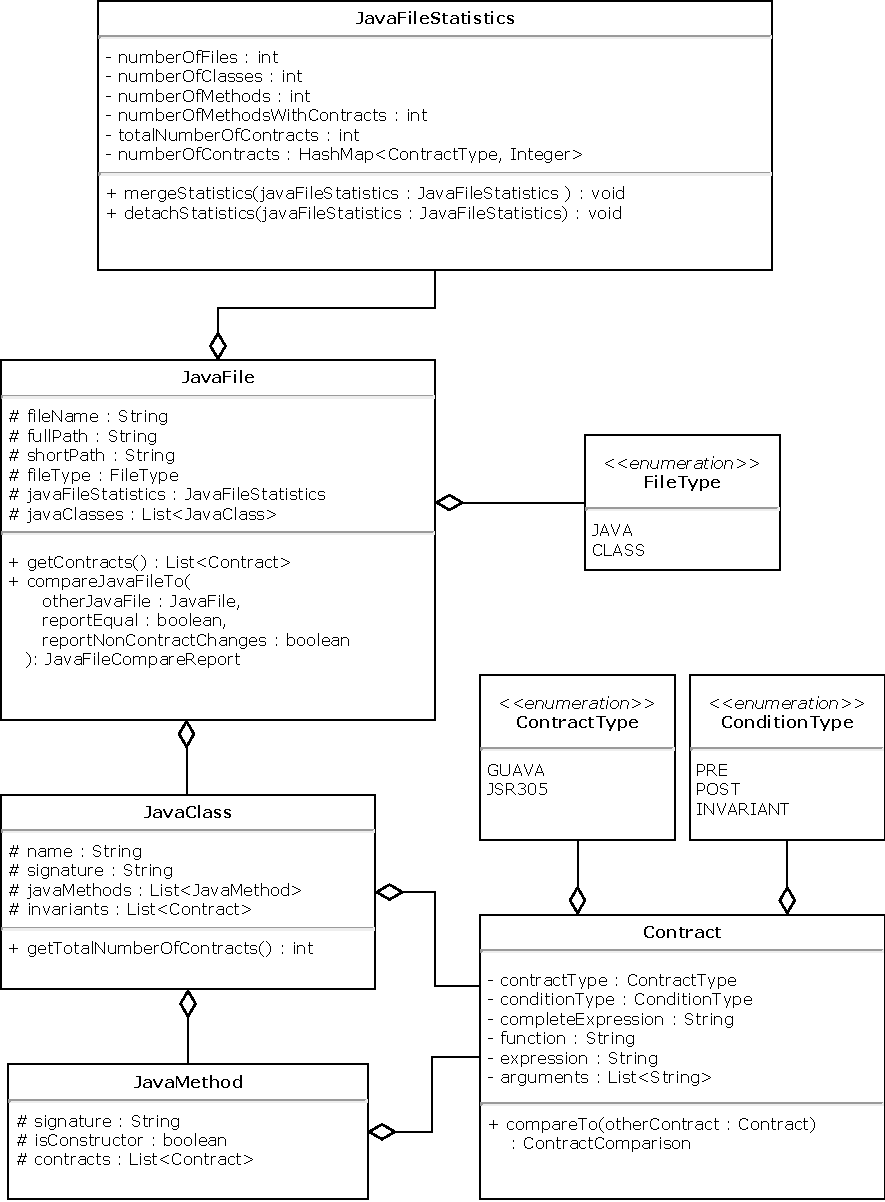
\includegraphics[width=1\textwidth]{img/modelExtractorDiagram.pdf}
						\caption[modelExtractorDiagram]{UML diagram datového modelu}
						\label{modelExtractorDiagram}
					\endminipage\hfill
				\end{figure}


	\section{Model pro porovnávání kontraktů}
		TODO
	
	\section{Diagram modelu pro porovnávání kontraktů}
		TODO

			
		\section{Externí reprezentace modelu}
			Pro externí reprezentaci modelu jsem zvolil použití formátu JSON. Tento formát je široce používaný zápis dat a umožňuje relativně snadné ukládaní objektů typu Java. JSON je tak vhodný pro zpracovaní strojem, ale je dobře čitelný i pro lidské oko (v případě, že byl zformátován). Díky těmto kvalitám je JSON vhodným formátem pro zobrazení, archivaci i další zpracování extrahovaných dat.\\
			
			Alternativou bylo použití formátu XML. Tento formát má v podstatě stejné přednosti jako JSON, s tím rozdílem, že obvykle není potřeba dalšího formátování proto, aby byl čitelný pro člověka, nicméně je oproti formátu JSON více opsaný. I přesto, že XML by byla také validní možnost pro reprezentaci dat, po dohodě s vedoucím práce jsme se rozhodli pro použití JSON. Důvodem byla zejména jeho stručnost, ale také lepší vlastnosti pro předávání mezi jinými nástroji.